% Essential Formatting

\documentclass[12pt]{article}
\usepackage{epsfig,amsmath,amsthm,amssymb}
%\usepackage[questions, answersheet]{urmathtest}[2001/05/12]
%\usepackage[answersheet]{urmathtest}[2001/05/12]
\usepackage[answers]{urmathtest}[2001/05/12]


% For use with pdflatex
% \pdfpagewidth\paperwidth
% \pdfpageheight\paperheight

% Basic User Defs

\def\ds{\displaystyle}

\newcommand{\ansbox}[1]
{\work{
  \pos\hfill \framebox[#1][l]{ANSWER:\rule[-.3in]{0in}{.7in}}
}{}}

\newcommand{\ansrectangle}
{\work{
  \pos\hfill \framebox[6in][l]{ANSWER:\rule[-.3in]{0in}{.7in}}
}{}}


% Beginning of the Document

\begin{document}
\examtitle{LINEAR REGRESSION MODELS W4315}{HOMEWORK 2}{09/16/2009}
 \begin{center}
  Instructor: Frank Wood
 \end{center}
%%\studentinfo
\instructions{
  %\textbf{Circle your Instructor's Name along with the Lecture Time:}



  \begin{itemize}
  \item
    \textbf{Please show all your work.
            You may use back pages if necessary.}
  %\item
   % \textbf{Please put your \underline{simplified}
   %         final answers in the spaces provided.}
  \end{itemize}
}
\finishfirstpage

% Problems Start Here % ----------------------------------------------------- %


\problem{35} {
  Consider a simple linear regression model $Y=\beta_0+\beta_1X+\epsilon$. $X$ takes value at all the integers from 1 to 20. We denote the ordinary least squared estimates of $\beta_0$ and $\beta_1$ as $b_0$ and $b_1$. Now assume that $\beta_0=2$, $\beta_1=0.3$ and $\sigma^2=4$.\\

 a. What are the exact distributions of $b_0$ and $b_1$?

 b. Generate $Y$ according to the given model (there are 20 $X$'s, so you need to generate 20 $Y$'s), and calculate the OLS estimates $b_0$ and $b_1$ based on $X$ and the simulated $Y$. Repeat the process 1,000 times and you will have 1,000 estimates of $\beta_0$ and $\beta_1$. For each parameter, draw a density histogram of the estimates.

 c. Superimpose the $b_0$ and $b_1$'s probability density functions onto the two histograms respectively. Is the histogram a
 close approximation of the curve?
   }
 { \vfill
  \answer
}
{
a. $b_0 \sim N(0.3, 4*(1/20+10.5^2/665)=0.863)$, $b_1 \sim N(2, 4/665=0.006)$\\
b.c. The histogram and the density function curve should be the same.
}


\problem{25} {
Write a matlab function to produce the ANOVA table as in TABLE 2.2 page 67 of the textbook. Specifically, the interface of your function must be

\begin{center}                function [SSR, SSE, SSTO, df\_R, df\_E, df\_TO] = anova\_1d(X, Y)
\end{center}

This function accepts $X$ and $Y$ as arguments and returns $SSR$, $SSE$, $SSTO$ and their associated degrees of freedom. Please complete the function defined in the file ``anova\_1d.m'' that you can find on the homework section of the course website. We have provided you the exact function interface in that file. (As in homework 1, you are only allowed to use basic matlab commands to write this function. )

  }
 { \vfill
  \answer
} {Use your own test data to test the validity of their programs.}

\problem{40} {
  Use the data in the file ``problem3.txt'' on the course website. This is a 20 by 2 matrix, with the first column being $X$ and second column being $Y$. Assume a simple linear regression model.\\
 a. Give the ordinary least square estimates of $\beta_0$, $\beta_1$ and $\sigma^2$. Draw a scatterplot of the raw data and overlay the fitted line on it.

 b. F-test is used to test the linear relationship between $X$ and $Y$. Calculate the F-test statistic and p-value. Draw the probability density function of F distribution with appropriate degrees of freedom. What does the p-value mean on the graph?

 c. Write your own function to calculate p-value of F-test. The interface of your function must be:

\begin{center}
function p\_value = p\_value\_of\_F\_test(X, Y)
\end{center}

It takes $X$ and $Y$ as arguments and return p-value. Please implement the function defined in ``p\_value\_of\_F\_test.m'' that you can find on the homework section of the course website. We have provided you the exact function interface in that file. (As before, you are only allowed to use basic matlab commands.)
}
 { \vfill
  \ANSWER
} {
a. The estimates are $\hat{\beta}_0 = 2.95$, $\hat{\beta}_1 = 0.16$, $\hat{\sigma}^2 = 1.34.$\\
b. F-statistic is 3.373 with degrees of freedom 1 and 18. The p-value is 0.083. The meaning
of p-value is the area under the density curve that is to the right of the F statistic.\\
c. Use the data 'problem3.txt' to test the program. It should return the correct p-value
0.083.
\begin{figure}[!h]
\begin{center}
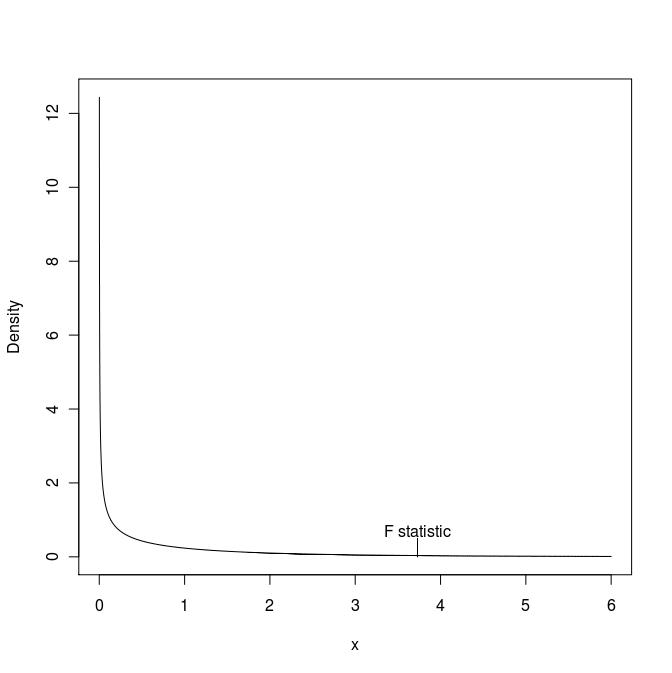
\includegraphics[width=.8\textwidth]{plot.jpg}
\end{center}
\end{figure}
}


% Problems End Here % ------------------------------------------------------- %

\problemsdone
\end{document}

% End of the Document
